\documentclass[9pt, aspectratio=43]{beamer}

\usepackage{amsmath}
\usepackage{booktabs}
\usepackage{color}
\usepackage{csquotes}
\usepackage{fontspec}

%%%%%%%%%%%%%%%%%%%%%%%%%%%%%%%%%%%%%%%%%%%%%%%%%%%%%%%%
% Theme
%%%%%%%%%%%%%%%%%%%%%%%%%%%%%%%%%%%%%%%%%%%%%%%%%%%%%%%%

\usetheme[progressbar=frametitle]{metropolis}
\metroset{block=fill}
\metroset{sectionpage=progressbar}
\usefonttheme{professionalfonts}
\usepackage{theme/beamercolorthememetropolisinria}

%%%%%%%%%%%%%%%%%%%%%%%%%%%%%%%%%%%%%%%%%%%%%%%%%%%%%%%%
% Syntax highlighting
%%%%%%%%%%%%%%%%%%%%%%%%%%%%%%%%%%%%%%%%%%%%%%%%%%%%%%%%

\usepackage{minted}
\definecolor{codebg}{rgb}{0.95, 0.955, 0.96}

\setminted[bash]{
    autogobble,
    baselinestretch=1.2,
    bgcolor=codebg,
    fontsize=\footnotesize,
    framesep=50mm,
    xleftmargin=1em,
    xrightmargin=1em,
}

\setminted[python]{
    autogobble,
    baselinestretch=1.2,
    bgcolor=codebg,
    fontsize=\footnotesize,
    framesep=50mm,
    xleftmargin=0.5em,
    xrightmargin=0.5em,
}

%%%%%%%%%%%%%%%%%%%%%%%%%%%%%%%%%%%%%%%%%%%%%%%%%%%%%%%%
% Bibliography
%%%%%%%%%%%%%%%%%%%%%%%%%%%%%%%%%%%%%%%%%%%%%%%%%%%%%%%%

\usepackage[
    style=alphabetic,
    maxbibnames=99,
    maxcitenames=99,
]{biblatex}
\addbibresource{refs.bib}

%%%%%%%%%%%%%%%%%%%%%%%%%%%%%%%%%%%%%%%%%%%%%%%%%%%%%%%%
% Footnotes
%%%%%%%%%%%%%%%%%%%%%%%%%%%%%%%%%%%%%%%%%%%%%%%%%%%%%%%%

\newcommand\blfootcite[1]{%
    \invisible<1>{%
        {\color{white} \footfullcite{#1}}%
    }%
}

\newcommand\blfootcitetext[1]{%
    \invisible<1>{%
        \addtocounter{footnote}{-1}% assumes a footnotemark
        {\color{white} \footfullcite{#1}}%
    }%
}

\newcommand\blfootnote[1]{%
  \begingroup
  \renewcommand\thefootnote{}%
  \footnote{#1}%
  \addtocounter{footnote}{-1}%
  \endgroup
}

\newcommand\blfootnotetext[1]{%
  \begingroup
  \footnotetext{#1}%
  \endgroup
}

%%%%%%%%%%%%%%%%%%%%%%%%%%%%%%%%%%%%%%%%%%%%%%%%%%%%%%%%
% Abbreviations
%%%%%%%%%%%%%%%%%%%%%%%%%%%%%%%%%%%%%%%%%%%%%%%%%%%%%%%%

\def\eg{{\emph{e.g.}}}
\def\etal{{\emph{et al.}}}
\def\ie{{\emph{i.e.}}}
\def\xid{\dot{\xi}}

%%%%%%%%%%%%%%%%%%%%%%%%%%%%%%%%%%%%%%%%%%%%%%%%%%%%%%%%
% Metadata
%%%%%%%%%%%%%%%%%%%%%%%%%%%%%%%%%%%%%%%%%%%%%%%%%%%%%%%%

\title{
    Reinforcement learning for legged robots
}

\author{\textbf{St\'ephane Caron}}
\date{December 8, 2023}
\institute{Inria--\'{E}cole normale sup\'{e}rieure}

\begin{document}

\maketitle

%%%%%%%%%%%%%%%%%%%%%%%%%%%%%%%%%%%%%%%%%%%%%%%%%%%%%%%%%%%%%%%%%%%%%%%%%%%%%%%%

\begin{frame}{Terminology}
    ...
\end{frame}

\begin{frame}{Optimal control and RL}
    ...
\end{frame}

\begin{frame}{Policy gradient theorem}
    ...
\end{frame}

\begin{frame}{The Gymnasium API}
    \begin{itemize}
        \item Widespread, not necessarily the best one out there
    \end{itemize}
\end{frame}

\begin{frame}{Domain randomization}
    ...
\end{frame}

\begin{frame}{Reward vocabulary}
    Let $r_e$ denote the reward associated with an error function $e$:

    Motivation:
    \begin{itemize}
        \item Exponential: $r_e = \exp(-e^2)$
    \end{itemize}

    Penalization:
    \begin{itemize}
        \item Absolute value $r_e = -|e|$
        \item Squared value: $r_e = -e^2$
    \end{itemize}
\end{frame}

\begin{frame}{Environment bounds}
    \begin{figure}
        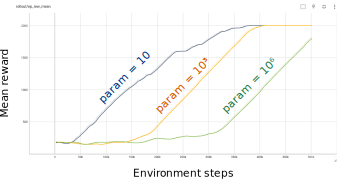
\includegraphics[width=\columnwidth]{genfig/max-accel.pdf}
    \end{figure}
\end{frame}

\begin{frame}{Caveat: stochastic}
    \begin{figure}
        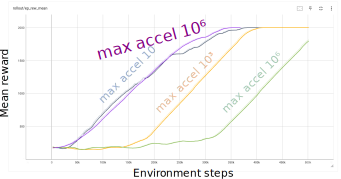
\includegraphics[width=\columnwidth]{genfig/max-accel-bis.pdf}
    \end{figure}
\end{frame}

\begin{frame}{Normalizing observations}
    \begin{itemize}
        \item Normalizing:
        \item Standardizing: 
    \end{itemize}
\end{frame}

\begin{frame}{Normalizing observations}
    not always a good thing! see figure
\end{frame}

\begin{frame}{That's all folks!}
    \vspace{2em}
    \begin{figure}
        \centering
        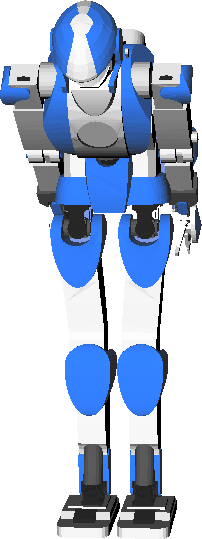
\includegraphics[height=10em]{genfig/thanks.pdf}
    \end{figure}
\end{frame}

%%%%%%%%%%%%%%%%%%%%%%%%%%%%%%%%%%%%%%%%%%%%%%%%%%%%%%%%%%%%%%%%%%%%%%%%%%%%%%%%

\section*{Bibliography}

\renewcommand*{\bibfont}{\footnotesize}
\setbeamertemplate{bibliography item}{\insertbiblabel}
\begin{frame}[allowframebreaks]{References}
    \printbibliography[heading=none]
\end{frame}

\section*{Templates}

\begin{frame}[fragile]{Python code}
    Load a robot description:
    \begin{minted}{python}
        from robot_descriptions.loaders.pinocchio import load_robot_description

        robot = load_robot_description("upkie_description")
    \end{minted}
    Visualize it:
    \begin{columns}
        \begin{column}{0.75\columnwidth}
            \begin{minted}{python}
                from pinocchio.visualize import MeshcatVisualizer

                robot.setVisualizer(MeshcatVisualizer())
                robot.initViewer(open=True)
                robot.loadViewerModel()
                robot.display(robot.q0)
            \end{minted}
        \end{column}
        \begin{column}{0.24\columnwidth}
            \begin{figure}
                \centering
                % \includegraphics[width=\columnwidth]{figures/upkie_description.png}
            \end{figure}
        \end{column}
    \end{columns}
    \blfootnote{
        Setup: \mintinline{bash}{pip install meshcat pin robot_descriptions}
    }
\end{frame}

\end{document}
